%LaTeX Curriculum Vitae Template
%
% Copyright (C) 2004-2009 Jason Blevins <jrblevin@sdf.lonestar.org>
% http://jblevins.org/projects/cv-template/
%
% You may use use this document as a template to create your own CV
% and you may redistribute the source code freely. No attribution is
% required in any resulting documents. I do ask that you please leave
% this notice and the above URL in the source code if you choose to
% redistribute this file.

\documentclass[letterpaper]{article}
\usepackage{graphicx}

\usepackage{hyperref}
\hypersetup{
    bookmarks=true,         % show bookmarks bar?
    unicode=false,          % non-Latin characters in Acrobat’s bookmarks
    pdftoolbar=true,        % show Acrobat’s toolbar?
    pdfmenubar=true,        % show Acrobat’s menu?
    pdffitwindow=true,     % window fit to page when opened
    pdfstartview={FitH},    % fits the width of the page to the window
    pdftitle={My title},    % title
    pdfauthor={Author},     % author
    pdfsubject={Subject},   % subject of the document
    pdfcreator={Creator},   % creator of the document
    pdfproducer={Producer}, % producer of the document
    pdfkeywords={keyword1} {key2} {key3}, % list of keywords
    pdfnewwindow=true,      % links in new window
    colorlinks=true,       % false: boxed links; true: colored links
    linkcolor=blue,          % color of internal links (change box color with linkbordercolor)
    citecolor=blue,        % color of links to bibliography
    filecolor=blue,      % color of file links
    urlcolor=blue           % color of external links
}



\usepackage{geometry}
\usepackage{import} % To import email.
\usepackage{marvosym} % face package
%\usepackage{xcolor,color}
\usepackage{fontawesome}
\usepackage{amssymb} % for bigstar
\usepackage{epigraph}
\usepackage{float}
\usepackage[svgnames]{xcolor}

% Comment the following lines to use the default Computer Modern font
% instead of the Palatino font provided by the mathpazo package.
% Remove the 'osf' bit if you don't like the old style figures.
\usepackage[T1]{fontenc}
\usepackage[sc,osf]{mathpazo}

% Set your name here
\def\name{Research Plan}

% Replace this with a link to your CV if you like, or set it empty
% (as in \def\footerlink{}) to remove the link in the footer:
\def\footerlink{}
% \href{http://www.hectorbahamonde.com}{www.HectorBahamonde.com}

% The following metadata will show up in the PDF properties
\hypersetup{
  colorlinks = true,
  urlcolor = blue,
  pdfauthor = {\name},
  pdfpagemode = UseNone
}

\geometry{
  body={6.5in, 8.5in},
  left=1.0in,
  top=1.25in
}

% Customize page headers
\pagestyle{myheadings}
\markright{{\tiny \name}}
\thispagestyle{empty}

% Custom section fonts
\usepackage{sectsty}
\sectionfont{\rmfamily\mdseries\Large}
\subsectionfont{\rmfamily\mdseries\itshape\large}

% Don't indent paragraphs.
\setlength\parindent{0em}

% Make lists without bullets
\renewenvironment{itemize}{
  \begin{list}{}{
    \setlength{\leftmargin}{1.5em}
  }
}{
  \end{list}
}


%%% bib begin
\usepackage[american]{babel}
\usepackage{csquotes}
%\usepackage[style=chicago-authordate,doi=false,isbn=false,url=false,eprint=false]{biblatex}

\usepackage[authordate,isbn=false,doi=false,url=false,eprint=false]{biblatex-chicago}
\DeclareFieldFormat[article]{title}{\mkbibquote{#1}} % make article titles in quotes
\DeclareFieldFormat[thesis]{title}{\mkbibemph{#1}} % make theses italics

\AtEveryBibitem{\clearfield{month}}
\AtEveryCitekey{\clearfield{month}}

\addbibresource{/Users/hectorbahamonde/Bibliografia_PoliSci/library.bib} 
\addbibresource{/Users/hectorbahamonde/Bibliografia_PoliSci/Bahamonde_BibTex2013.bib} 

% USAGES
%% use \textcite to cite normal
%% \parencite to cite in parentheses
%% \footcite to cite in footnote
%% the default can be modified in autocite=FOO, footnote, for ex. 
%%% bib end




\begin{document}

% Place name at left
%{\huge \name}

% Alternatively, print name centered and bold:
\centerline{\huge \bf \name}

%\epigraph{\emph{Statistics: ``science dealing with data about the condition of a state or community''}}{Gottfried Aschenwall, 1770}


\vspace{0.25in}

\begin{minipage}{0.45\linewidth}
 University of Turku \\
 \href{https://invest.utu.fi}{INVEST Research Flagship Centre} \\
  Turku, Finland\\
  \\
  \\

\end{minipage}
\hspace{4cm}\begin{minipage}{0.45\linewidth}
  \begin{tabular}{ll}
{\bf Hector Bahamonde, PhD}\\
{\color{blue}{\bf Senior Researcher}}\\
\href{https://invest.utu.fi/welfare-research-and-ecosystem/investhub/}{INVESThub}\\%\\
   %{\bf {\color{red}{\scriptsize Not intended as a definitive version}}} %\\
 \texttt{e:}\href{mailto:hector.bahamonde@utu.fi}{\texttt{hector.bahamonde@utu.fi}}   \\
 \texttt{w:}\href{http://www.hectorbahamonde.com}{\texttt{www.HectorBahamonde.com}}   \\
    \\
    \\
    \\
  \end{tabular}
\end{minipage}

%\vspace{5mm}
%{\bf TA}: Valtteri Pulkkinen.\\
%\texttt{e}: \href{mailto:valtteri.s.pulkkinen@utu.fi}{\texttt{valtteri.s.pulkkinen@utu.fi}}\\
%{\bf TA Bio}: He is a soon-to-be MA in Political Science and the TA for this course. Pulkkinen is especially interested in quantitative methods, private-public cooperation and public affairs. You can email him for help before and during this course.\\



\vspace{-10mm}

\subsection*{Overview}

Democracy faces a crisis with the rise of populist, far-right, and far-left parties \parencite{Mudde2004,Coffe2007a}. My project seeks to unravel the reasons behind the electoral success of these movements. My argument is that, as economic inequality rises, the perceived potential losses for the less well-off intensify, leading to increased support for populist, far-right, and far-left parties. Conceptually, voters adjust their reference points due to declining economic prospects, while populist parties tap into the heightened loss aversion of voters. While the inequality hypothesis has been previously introduced, there are two important shortcomings. Conceptually, previous works have overlooked the idea of ``loss aversion'' \parencite{Kahneman1979}, a critical miss, especially when studying the political effects of economic \emph{losses} and \emph{inequality}. For example, while most scholars concentrate on \emph{diminishing} levels of status \parencite{Gidron2017a} or \emph{decreasing} material well-being \parencite{Oesch2008a}, the literature often misses the fact that \emph{individuals are more sensitive to losses than equivalent gains} \parencite[p. 171]{Levy1992a}. Considering the \emph{asymmetrical} political effects of losses and gains, can reversing the same levels of inequality that caused populism also ``\emph{un-cause}'' it? Unfortunately, the literature has missed these kinds of questions. Furthermore, the inequality hypothesis has not been rigorously tested \parencite[p. 154]{Engler2021}. For instance, \textcite{Rooduijn2018b} analyzes 15 key populist parties across \emph{11} Western European democracies only to find that a populist voter type does not exist. I attribute these kinds of oversights to scholars \emph{missing a focus on loss aversion} and also \emph{relying on survey methods with observational data} that are susceptible to social desirability biases \parencite{Kuklinski1997}. 

\vspace{2mm}In general, the literature is in very bad shape, not only lacking conclusive answers \parencite[p. 6]{Ivarsflaten2008}, but also offering a \emph{cacophony} of clashing explanations. Some assert that ``No, people really aren't turning away from democracy'' \parencite{Voeten2016}, yet others counter with ``Yes, people really are turning away from democracy'' \cite{Mounk2016}. And while some studies resonate with my income inequality hypothesis \parencite{Han2016b}, others emphasize social status while specifically \emph{disregarding} economic inequality \parencite{Gidron2017a,Oesch2008a}. {\bf In fact, the misunderstanding in the literature is so profound that some even claim that high inequality \emph{reduces} support for far-right parties} \parencite[p. 725]{Patana2020b}, while others \emph{dismiss} economic factors altogether with remarks like ``it's \emph{not} the economy, stupid!'' \parencite{Mudde2007b}.\footnote{Emphasis in original.}

\vspace{2mm}Amidst this confusion, my research offers a novel {\bf substantive contribution} to the literature. Drawing from our research \parencite{Bahamonde2022b}, I introduce prospect theory \parencite{Kahneman1979} to the study of extremist politics. Several reasons make this theory particularly apt for understanding extreme political tendencies. First, prospect theory elucidates decision-making amidst \emph{risk} \parencite{McDermott1998,Levy1992a}, both political and economic. Politically, the \emph{unpredictability} of novice populist parties \parencite{Ivarsflaten2008} makes voting for them a risky decision. Economically, many describe extreme voters as the ``\emph{losers} of globalization'' \parencite{Im2019,Milner2021b}, situating voters in a globalization-induced unemployment risk.  Thus, since ``\emph{losses loom larger than gains}'' \parencite{Kahneman1979}, understanding the asymmetric political consequences amidst rising economic inequality levels---as addressed in our own work, i.e., \parencite{Bahamonde2021}---becomes vital. Yet, the literature overlooks how voting for populist parties is a risky strategy itself aimed at ``recovering losses [...] to aggressively compensate for prior losses'' (as discussed in our work; e.g., \cite[p. 2]{Bahamonde2022b}). Second, unlike personality theories, prospect theory does \emph{not} require knowing individual personality traits for predicting behavior \parencite{McDermott2004,Vis2011}. This stands in contrast to personality-driven theories of radical support \parencite{Cohen2016} which face substantial causality concerns \parencite{Mudde2007b}. In practice, prospect theory promises to address many previously overlooked questions: Do far-left and far-right movements \emph{frame} social and economic \emph{losses} differently (i.e., ``\emph{framing effects},'' \cite{Kahneman1979})? At what threshold of inequality do voters reach an indifference point towards extremist movements?

\vspace{2mm}Moving forward, I also make several {\bf novel methodological contributions} to the literature. The literature heavily relies on survey research, which has very important shortcomings: causal factors are obscured (King et al. 1994), datasets usually lack statistical representativeness of extreme-party supporters (Mudde 2007), and self-reported preferences towards ``democracy'' have their own set of challenges because not everyone has a uniform understanding of what ``democracy'' is or implies (Ananda 2021). It is particularly crucial to address these biases as many of the extreme parties in question back policies that are not widely accepted by society, such as restricting immigration or limiting humanitarian aid (Dehdari 2022, p. 194, and Betz 1993 p. 413), which are themselves significantly influenced by social desirability biases (Kuklinski 1997). For example, using experimental methods, Klar et al. (2016) find that Trump supporters are more likely to conceal their support for him, while Brownback and Novotny (2018) find that Democrats are more likely to lie about their agreement with some of Trump's policies. Despite these findings, the broader literature often neglects the benefits of experimental methods. My project addresses these causal inference and bias issues by using experimental designs, register data, and sophisticated econometric techniques. 

{\color{red}This Research Plan comprises {\bf two main activities} that will take place between 2024 and 2028} (see \autoref{fig:1}).

\subsection*{Research Activities: 2024---2028}

\paragraph{First activity.} Most research focuses on voters. For example, some studies indicate that income inequality pushes poorer \emph{voters} towards radical parties \parencite{Han2016b}. However, others argue that \emph{voters}' social status (but \emph{not} income inequality) plays a more pivotal role \parencite{Gidron2017a,Oesch2008a}. Three key takeaways emerge from the existing literature. First, there is no clear consensus on what primarily drives extreme voting (\cite[p. 3]{Ivarsflaten2008}; \cite[p. 279]{Jesuit2009}). Second, most studies tend to have a static perspective, often concentrating on fixed moments and neglecting dynamic factors like shifts in status or inequality \parencite{Kurer2019}. This oversight is significant, as most theories, despite highlighting different factors, emphasize the importance of changes, whether in status or material well-being. Yet, scholars often fail to address these dynamic losses, both in theory and practice. Third, and as I have argued before \parencite{Bahamonde2020a}, the role of \emph{political candidates} remains underexplored. Do candidates \emph{resemble} the socio-economic backgrounds of the platforms they aspire to represent? Have \emph{their} socio-economic positions evolved over time? Integrating prospect theory provides a more comprehensive understanding, particularly in deciphering the interplay of dynamic changes \parencite[643]{Thaler1990} in status or material well-being and their influence on political behavior.

% PENDING BELOW
\vspace{2mm}I concentrate on the intersection of supply (candidates) and demand (voters) for far-right populist ideas and incorporate two types of survey experiments: {\bf list experiments}, as explained in my own work \parencite{Bahamonde2020a}, and {\bf conjoint experiments} \parencite{Hainmueller2014}. The list experiment is designed to elicit truthful responses to sensitive questions, while the conjoint experiment explores multidimensional choices and reduces social desirability bias. I aim to employ these techniques to examine (multidimensional) determinants of attitudes towards immigration, welfare redistribution, racism, and democratic support, spanning both voters and parties. These data will then be merged with macro-structural socio-economic variables. My goal is to study where the supply of populist ideas and demand for these ideas meet, a framework exemplified in the concept of (extreme) ``party-mass linkages'' as described by \textcite{Kitschelt2000}. 

% PENDING BELOW
\vspace{2mm}Importantly, I deviate from the customary approach in survey research which involves randomly sampling the entire population \parencite{Mudde2007b}. Instead, I survey \emph{genuine} supporters of the Finns Party. Exploiting the fact that the party charges a membership fee in exchange for which party members receive the party's magazine in their mailbox, I will utilize the state-owned postal service mailer service, accessible to standard marketing companies in Finland. From this, I will send invitation letters to a random sample of actual party supporters to participate in the two aforementioned longitudinal survey experiments (\emph{n}=1000). Using a similar experimental design and questioner, the project also seeks to collect data from current and former Finns Party candidates and politicians. Drawing from our previous work \parencite{Bahamonde:2023}, we will utilize rich Finnish register-level data. From this data, postcards will be sent to a random selection of \emph{n}=200 candidates, inviting them to participate in the two aforementioned longitudinal survey experiments. I intend to carry out 3 surveys annually for 5 years (2024 till 2028), resulting in a total of 15 surveys each for both politicians and supporters (see \autoref{fig:1}).

% PENDING BELOW
\vspace{2mm}Furthermore, the individual-level longitudinal data (supporters and politicians) will be merged with longitudinal district-level data, such as overtime measures of inequality, immigration, among others \parencite{Dehdari2022,Kurer2019,Gidron2020}. This integration aims to provide insights into the underlying motivations fueling support for radical far-right politics. This design is advantageous for dynamic causal identification, allowing the tracking of real-world changes \parencite{Im2023}.

\paragraph{Second activity.} The main objective of this activity explores the formation process behind extremist attitudes. This is a crucial aspect to consider. Some suggest that the roots of radical voting lie in personality traits. For example, \textcite[p. 1]{Cohen2016} argue that authoritarianism is a personality trait. While their findings are compelling, they raise serious questions about endogeneity. This line of thought stems from Adorno's ``The Authoritarian Personality'' (\citeyear{Adorno1950}): those brought up by an authoritarian father are predisposed to authoritarian attitudes \parencite{Helminen2023}. However, this theory struggles to explain the \emph{recent} rise in extreme support, \emph{unless conservative families in the 1960s had more children} \parencite[p. 218]{Mudde2007b}. To solve this issue, I will test the explanatory power of my loss-focused inequality hypothesis against the personality hypothesis. Additionally, I will test other explanations that touch upon issues related to material deprivation, such as the cultural \parencite{Engler2021,Veugelers2002}, social \parencite{Gidron2017a}, ethnic \parencite{Helske2023}, democratic values \parencite{Lipset1981,Carlin2015}, and ``negative partisanship'' \parencite{Mudde2018} hypotheses. Incorporating prospect theory offers a distinct advantage as it allows for predictive insights into voting behavior without necessitating an understanding of individual personality traits, bridging the gap between economic and personality explanations.

% PENDING BELOW
\vspace{2mm}The methodological contribution of this activity is to implement a novel longitudinal lab (voting) experiment designed to study the decision-making process driving support for populist far-right and far-left movements. Economic lab experiments allow for the direct observation of participant behavior. By setting up specific scenarios, researchers can gain insights into how individuals make choices \parencite{Kahneman:2012tc}. My experiment will take place at the {\bf PCRC Decision Making Laboratory at the University of Turku}, the oldest decision-making lab in Finland.  Importantly, the lab already maintains a panel of Finnish citizens, eliminating recruitment needs. 

% PENDING BELOW
\vspace{2mm}The study is structured in \emph{t}=10 waves, each spaced about two to three weeks apart. All \emph{n}=200 participants will assume the role of a ``citizen,'' and all will be compensated to participate in the 10 waves. To simulate the \emph{market dynamics} influencing radical voting, in wave \emph{t}=1 they will be given a hypothetical occupational status (which they will retain for the remaining 9 waves). These statuses include various job types with their corresponding hypothetical monthly post-tax incomes. Due to infrastructural and computational limitations, I can accommodate only 40 participants in each session, leading to 5 experimental sessions per wave. I intend to spend one whole week per wave (see \autoref{fig:1}). This approach allows me to simulate different societal structures with diverse income distributions between each experimental session.  As the experiment unfolds, participants encounter a series of exogenous shocks (experimental conditions), e.g., spikes in unemployment, crime, or immigration. Finally, participants will be exposed to different ``campaigns'' (vignettes) from (fictional) political candidates. These ``campaigns'' will mirror messages typical of populist/extremist platforms \parencite{Schumacher2022}, as well as those of traditional left, center, and right candidates. In the final 10th wave, participants will individually have the opportunity to cast their ballots for one of these candidates. 

% PENDING BELOW
\vspace{2mm}Importantly, I will include different questions frequently used in studies focused on the ``authoritarian personality.'' This includes the ``fascism'' \parencite{Altemeyer1981}, the ``child-rearing values'' \parencite{Helminen2023} and the ``right-wing authoritarianism'' \parencite{Duckitt2013a,Feldman2003,Hetherington2009} scales. This will enable me to better understand the complex interplay between income inequality and personality-based explanations of radical voting. 

\subsection*{Expected Outcomes and Impact}

My project is expected to have the following expected contributions:

\begin{itemize}

  \item {\bf Academic Contributions}: 
    \begin{enumerate}
      \item {\bf Development of Theoretical Frameworks}: The project aims to contribute to the theoretical understanding of the relationship between economic inequality and political extremism. It seeks to refine existing models and possibly develop new ones that better capture this complex interplay.

      \item {\bf Empirical Contributions}: Through its innovative combination of experimental and survey methodologies, the project will provide robust empirical data. This data will be invaluable in testing and refining theories about economic inequality's impact on political attitudes and behavior.

      \item {\bf Methodological Advancements}: The project's methodological rigor and innovation are expected to set new standards in interdisciplinary research. The techniques developed could be applicable in broader contexts, enabling future studies to adopt similar methodologies for their research inquiries.
    \end{enumerate}

  \item {\bf Policy Implications}: 
    \begin{enumerate}
      \item {\bf Informed Policy Making}: By providing a deeper understanding of the root causes of extremism, the research can guide policymakers in developing strategies to counteract the rise of extremist parties. This could involve economic policies aimed at reducing inequality, as well as social policies designed to promote social cohesion and political stability.

      \item {\bf Addressing Economic Inequality}: The research will offer insights into how economic policies can be better tailored to address the underlying issues of inequality. This could lead to more effective economic reforms that are sensitive to their political implications.

      \item {\bf Educational and Social Programs}: The project's findings could inform educational and social programs aimed at promoting democratic values and critical thinking, particularly in communities most affected by economic disparities.
    \end{enumerate}

  \item {\bf Societal Impact}: 
    \begin{enumerate}
      \item {\bf Enhanced Public Understanding}: Disseminating the findings in accessible formats will enhance public understanding of the connections between economic conditions and political leanings. This increased awareness is crucial in an era marked by political polarization and economic uncertainty.
      \item {\bf Strengthening Democratic Processes}: By identifying factors that lead to the rise of extremism, the project can contribute to the strengthening of democratic processes. Understanding these dynamics is crucial for building resilient democracies that can withstand economic and political challenges.
    \end{enumerate}

\end{itemize}

{\color{red}make sure I say it's all panel data.}

\subsection*{Timeline and Milestones}

The project consists of two main activities. Both of them follow similar stages (see \autoref{fig:1}). The project as a whole begins with the initial design and pre-testing phase, where the foundations of the research are laid out, followed by the commencement of data collection in multiple waves. This strategy ensures that data is collected in a manageable and methodical manner, allowing for timely analysis between waves, allowing for data analysis and the preparation for conferences and workshops. Midway through the timeline, there is an overlap between ongoing data collection waves and data analysis, where there will be a more intensive phase of the project where findings are beginning to be synthesized and disseminated on a preliminary basis. The final stages of the project are marked by an increase in dissemination activities, with a focus on writing and publishing papers. This marks a transition from active data collection to a period where the emphasis is on sharing the research findings with the broader academic community. The project exhibits a cyclical pattern of data collection, analysis, and dissemination, indicating a dynamic process that will likely foster a rich environment for refinement of the research objectives and outcomes.

\begin{figure}[h]
\caption{{\bf Gantt Chart: Research Plan between 2024 and 2028.}}
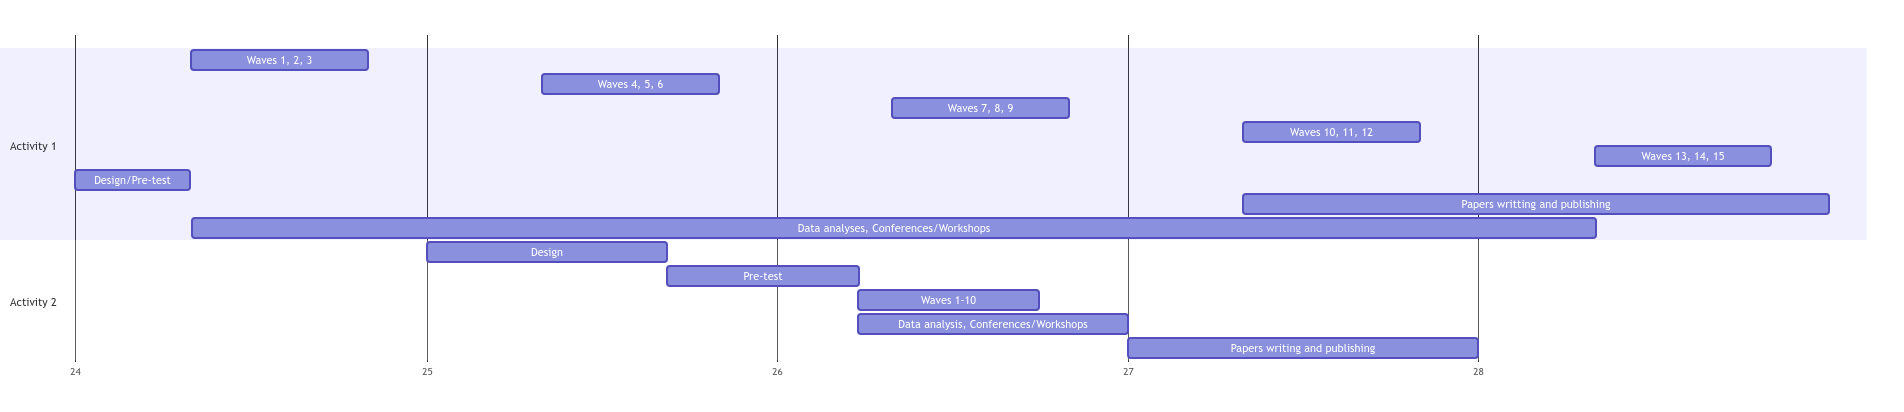
\includegraphics[width=\textwidth]{gantt.png} 
\label{fig:1}
\end{figure}


\subsection*{Budget and Resources}

The budget for this project has been meticulously planned to cover a comprehensive range of expenses, ensuring a robust and efficient execution of my research objectives. This includes the costs for experimental setups, data collection, and the postdocs salaries. Additionally, I have accounted for the dissemination of my findings through conferences and publications. Key resources such as access to laboratory spaces and advanced computational tools, post-docs, are integral to the success of this project. 

\vspace{2mm}By January 2024, four institutions will be reviewing my project for potential funding.\footnote{Kone Foundation (application \#202303858), Finnish Cultural Foundation (application \#575159CE), ERC ``Starting Grant'' (application \#101163663) and Research Council of Finland (not applied yet).} Given the project's innovative approach and its potential for significant contributions to the field and society, I am confident in my prospects of securing the necessary funds.


\subsection*{Conclusion}

My project promises to provide significant contributions to the understanding of the interplay between economic inequality and political extremism. Through its innovative methodological approach and comprehensive analysis, I aim to shed light on some of the most pressing political challenges facing modern democracies. The findings of this research are expected to have far-reaching implications, informing both academic discourse and practical policy-making in the realm of political economy and beyond.

\vspace{2mm}I kindly invite the InvestHub Selection Committee to take my re-application into consideration. Please feel free to contact me if you have any questions or need further information.



\newpage
%\pagenumbering{roman}
%\setcounter{page}{1}
\printbibliography



\end{document}


